%%% Clinic Template
%%%
%%% C.M. Connelly <cmc@math.hmc.edu>
%%%
%%%  $Id$


%%% !!! HMC STUDENTS SHOULD REMOVE THE FOLLOWING COPYRIGHT NOTICE FROM
%%% !!! FINAL SUBMISSIONS.

%%% Copyright (C) 2004-2010 Department of Mathematics, Harvey Mudd College.
%%%
%%% This file is part of the hmcclinic class document provided to
%%% HMC mathematics students.
%%%
%%% See the COPYING document, which should accompany this
%%% distribution, for information about distribution and 
%%% modification of the document and its components.

%%% !!! END COPYRIGHT NOTICE.


%%% Clinic reports use the clinic class, which should be located
%%% somewhere in TeX's search path.

%%% For your ``statement of work'' (or ``work statement''), specify
%%% the ``proposal'' document-class option to the hmcclinic class.
\documentclass[midyear]{cguclinic}

%%% There are also some changes in pagination styles and content
%%% that reflect the briefer nature of the proposal.  For example,
%%% in the longer reports, you use \frontmatter, \mainmatter, and
%%% \backmatter to separate some sections of the report from
%%% others.  In the statement of work, you don't need those
%%% commands, as no such division is necessary.

%%% Other packages needed by your document may be loaded here.
\usepackage{float}
\usepackage[T1]{fontenc}
\usepackage{fourier}
\usepackage[english]{babel}
\usepackage{amsmath,amsthm}
\usepackage{graphicx}
\usepackage[justification=justified]{caption}
\usepackage{subcaption}
\usepackage{comment}
\usepackage{amsthm}
\usepackage{tikz}
\usepackage{enumitem}
\usetikzlibrary{shapes,arrows}
\usetikzlibrary{calc}
\usetikzlibrary{positioning, decorations.pathmorphing, shadows,decorations.markings}
\usepackage{pgf,pgfarrows,pgfnodes,pgfautomata,pgfheaps,pgfshade,tikz}
\usetikzlibrary{arrows.meta, calc, chains, quotes, positioning, shapes.geometric, fit}
\usepackage{booktabs}


\theoremstyle{definition}
\newtheorem{definition}{Definition}
%%% The major difference between the statement of work and a midyear
%%% or final report is that the statement of work is typeset as an
%%% article, which means that the highest level of structural
%%% division available to you is section rather than chapter.

%%% There are also some changes in pagination styles and content
%%% that reflect the briefer nature of the proposal.  For example,
%%% in the longer reports, you use \frontmatter, \mainmatter, and
%%% \backmatter to separate some sections of the report from
%%% others.  In the statement of work, you don't need those
%%% commands, as no such division is necessary.

%%% Other packages needed by your document may be loaded here.
% \usepackage{url}              % For formatting URLs and other web or
                                % file references.

%%% Provide additional context around errors. 
\setcounter{errorcontextlines}{1000}


%% What is the name of the company or organization sponsoring your project?
\sponsor{Sandia National Laboratories}

%% What is the title of your report?
\title{Graph Theoretic Machine Learning Approaches to Predict Atomic Scale Fracture in Silica-Based Glasses}

%% Who are the authors of the report (your team members)?  (Separate
%% names with \and.)
\author{Shu Cheng \and Yuri Kim \and Adam Lawrence (Project Manager) \and Corina Oroz}

%% What is your faculty advisor's name?  (Again, separate names with
%% \and, if necessary.)
\advisor{Allon Percus}

%% Liaison's name or names?
\liaison{Mark Wilson \and Thomas Hardin}

%% Did you have an outside consultant help you with this project?  Put
%% their names in the \consultant command.
%\consultant{Joseph Jones}

\date{December 6, 2019}
% Uncomment to manually edit date. Commented, TeX will automatically insert today's date.

%%% End of information section.

%%% New commands and environments.

%%% You can define your own commands and environments here.  If you
%%% have a lot of material here, you might want to consider splitting
%%% the commands and environments into a separate ``style'' file that
%%% you load with \usepackage.

%\newcommand{\coolcommand}[1]{#1 is cool.} % Lets everyone know that
                                % the person or thing that you provide
                                % as the argument to the command is
                                % cool.


%%% Some theorem-like command definitions.

%%% The \newtheorem command comes from the amsthm package.  That
%%% package is loaded by the class file.

%%% Note that these definitions have changed from the version in the
%%% sample report document by dropping the ``within'' argument.  See
%%% Gratzer's _Math into LaTeX_ or the AMS-LaTeX documentation for
%%% more details.

% \newtheorem{thm}{Theorem}
% \newtheorem{Theo1}{Theorem}
% \newtheorem{Theo2}{Theorem}
% \newtheorem{Lemma}{Lemma}
\usepackage{url}


%%% If you find that some words in your document are being hyphenated
%%% incorrectly, you can specify the correct hyphenation using the
%%% \hyphenation command.  Note that words are separated by
%%% whitespace, as shown below.

%\hyphenation{ap-pen-dix wer-ther-i-an}


%%% The start of the document!

%% The document environment is the main environment in any LaTeX
%% document.  It contains other environments, as well as your text.

\begin{document}
\frontmatter

\maketitle

\abstract
Brittle materials are prevalent in industrial applications. A fundamental engineering challenge is predicting where failure can occur in such materials. This involves determining where fracture nucleation will occur, as well as how these fractures propagate.

Researchers at Sandia National Laboratories have successfully used molecular dynamics (MD) simulations to model the effects leading to fracture nucleation and growth in silica-based glasses, given an atomic-level description of the material. However, these simulations are too computationally intensive to allow a systematic study of the relation between atomic structure and fracture behavior.

This Clinic project develops a novel approach to predicting fracture growth in silicate glasses, using a graph theoretic description of the material and machine learning. By training a supervised learning algorithm on MD simulation data, we aim to develop a surrogate model that rapidly and accurately predicts where fractures will emerge under multiple environmental conditions. The model will provide new insight into how local structure, beyond a simple ``weakest link'' description, leads to fracture and failure.


\tableofcontents

\mainmatter

\chapter{Introduction}
\label{sec: Introduction}
\section{Sponsor}

The CGU Math Clinic project is sponsored by Sandia National Laboratories in Albuquerque, New Mexico. SNL is managed and operated by the National Technology and Engineering Solutions of Sandia, an owned subsidiary of Honeywell International, Inc. Originally founded in 1949, Sandia develops, engineers, and tests non-nuclear components of nuclear weapons, in response to federal government solicitations. Recent efforts at Sandia have involved studying fractures in silica-based glasses. In order to gain an improved understanding as to where and how fractures nucleate and propagate, Sandia aims to develop machine learning (ML) algorithms that will provide greater computational efficiency than the largely simulation-based approaches that are currently employed.

%%%Example from 20117-18 report%%%
%to further the US nuclear program, LANL's interest in modeling brittle damage centers around ensuring weapons safety and adherence to global nuclear testing standards by examining static fracture networks, modeling dynamic fracture propagation, and understanding uncertainty quantification and data assimilation. LANL currently has accurate, yet computationally intense methods of doing so. In the 2017-2018 project year, our focus is on modeling dynamic fracture propagation using Machine Learning (ML) methods based on LANL modeling data, to  reduce computational load dramatically while retaining that accuracy.

\section{Background}
Silicate glasses are used widely, in fields that include medicine, optics, electronics, telecommunication and energy. While these materials have numerous benefits in terms of strength and resilience, they are also brittle. When placed under sufficient tensile stress, glasses fracture rather than stretch. The fractures grow, propagating through the glass and ultimately leading to material failure. In spite of considerable study, the nanoscale origins of fracture and the relation of atomic structure to fracture nucleation remain poorly understood.

A natural hypothesis might be that fracture nucleation is related to the presence of atomic-scale defects or chemical bond weakness in the glass. However, the relationship between atomic structure and fracture behavior is complex. Fractures do not simply originate at the site of the weakest link or most easily broken bond, and trigger further fracturing in the surrounding bonds~\cite{markpres}. Similarly, glasses with an increased density of nanoscale voids and defects do not necessarily display increased brittle behavior, and can even be better at absorbing stresses from mechanical deformation~\cite{pedone2015dynamics}. Instead, the nucleation and propagation of fractures appear to depend on more subtle characteristics of the local structure surrounding an atom.

\subsection{Physical Structure}
The basic molecular unit in a silicate glass is a silicon (Si) atom bonded to four oxygen (O) atoms in a tetrahedral configuration.  Each of these SiO$_4$ units can share its O atoms with neighboring tetrahedra.  An O atom shared between two molecules in this way is known as a \emph{bridging oxygen}, as seen in Figure~\ref{fig:tetrahedra}.

\begin{figure}[!b]
    \centering
    \noindent
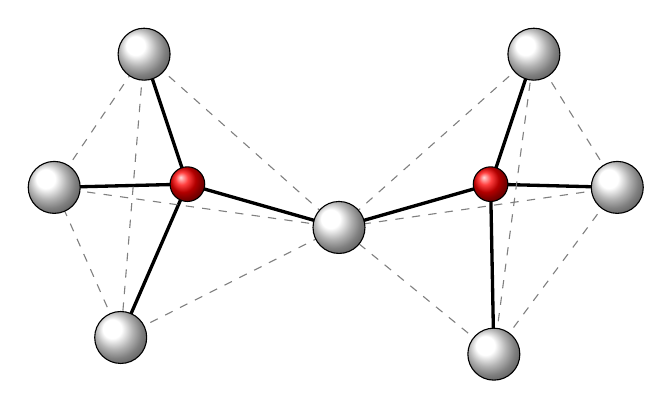
\begin{tikzpicture}[scale=1.1]
\coordinate (A) at (-0.5,0.5,0); % Left back O 
\coordinate (B) at (2,0.5,4.5); % Left front O  
\coordinate (C) at (6,0.5,0); % Right back O
\coordinate (D) at (6.5,0.5,5); % Right front O 
\coordinate (E) at (3.75,1,2.5); % Bridging Oxygen 
\coordinate (F) at (5.5,1.5,2.5); % Right Si
\coordinate (G) at (2,1.5,2.5); % Left Si 
\coordinate (H) at (1.5,3,2.5); % Left top O 
\coordinate (I) at (6,3,2.5); % Right Top O

%connections from left Si
\draw [very thick] (G) -- (A);
\draw [very thick] (G) -- (B);
\draw [very thick] (G) -- (H);
\draw [very thick] (G) -- (E);

%connections from Right Si 
\draw [very thick] (F) -- (C);
\draw [very thick] (F) -- (D);
\draw [very thick] (F) -- (I);
\draw [very thick] (F) -- (E);

%dashed lines between Oxygen. This can be removed but it was in literature. 
\draw[gray,dashed] (A) -- (H);
\draw[gray,dashed] (H) -- (B);
\draw[gray,dashed] (B) -- (A);
\draw[gray,dashed] (A) -- (E);
\draw[gray,dashed] (H) -- (E);
\draw[gray,dashed] (B) -- (E);

\draw[gray,dashed] (I) -- (C);
\draw[gray,dashed] (C) -- (D);
\draw[gray,dashed] (D) -- (I);
\draw[gray,dashed] (I) -- (E);
\draw[gray,dashed] (D) -- (E);                                                
\draw[gray,dashed] (C) -- (E);                                                

%place non-atom cube corners
\shadedraw [ball color= white] (A) circle (0.3cm);
\shadedraw [ball color= white] (B) circle (0.3cm);
\shadedraw [ball color= white] (C) circle (0.3cm);
\shadedraw [ball color= white] (D) circle (0.3cm);
\shadedraw [ball color= white] (E) circle (0.3cm);
\shadedraw [ball color= red] (F) circle (0.20cm);
\shadedraw [ball color= red] (G) circle (0.20cm);
\shadedraw [ball color= white] (H) circle (0.3cm);
\shadedraw [ball color= white] (I) circle (0.3cm);
\end{tikzpicture}
    \caption{Two silicon atoms (small red balls) with surrounding oxygen atoms (large grey balls) in tetrahedral configuration.  One bridging oxygen is at a corner shared by the two tetrahedra.}
    \label{fig:tetrahedra}
\end{figure}

When an Si atom is surrounded by $n$ bridging O atoms, it is called a Q$_n$ unit~\cite{shelby2005}. In a network of Q$_4$ units, all O atoms are shared between two Si atoms, forming a silicon dioxide (SiO$_2$) structure.  The network geometry can be regular, in which case the material is a crystal such as quartz.  Alternatively, the geometry can be irregular, in which case it is a glass.  When the network has Q$_n$ units with $n<4$, some of the O atoms surrounding an Si atom are non-bridging.

An Si atom can also be undercoordinated, bonding with fewer than four O atoms, or overcoordinated, breaking the tetrahedral symmetry and bonding with more than four O atoms.  In the latter case, this can result in rare Q$_n$ units with $n>4$~\cite{pedone2015dynamics}.

\subsection{Molecular Dynamics Simulations} 

The conventional approach for studying the fracture mechanics of materials has been to model their structure as a continuum, ignoring atomic detail, and predicting strength and failure using a theoretical description at the macroscopic scale.  For high-fidelity predictions of fracture dynamics in silica-based glasses, however, continuum theory encounters limitations~\cite{shimada2015breakdown}.

Molecular dynamics (MD) methods instead provide an atomistic approach, simulating the system at the nanoscale and modeling the individual chemical and physical interactions taking place in the material. These simulations have successfully predicted a wide range of detailed properties that cannot be obtained with continuum methods, and that are consistent with experimental observations~\cite{pedone2009properties}.

In order to model a silicate glass, MD simulates heating quartz to a very high temperature, far above its melting point.  The melt is then rapidly cooled, or \emph{quenched}, to room temperature, introducing the molecular disorder that characterizes glassy structure.  While the quench rate that can feasibly be simulated (3.7~K/picosecond) is orders of magnitude faster than experimental reality, it nevertheless provides results that are in many cases a good match with experimental data~\cite{markpres,mWilson_continuum_stress}

%%  CRACK PROPAGATION SIMULATION FIGURE 

\begin{figure}
    \centering
    \noindent
\hspace{6pt}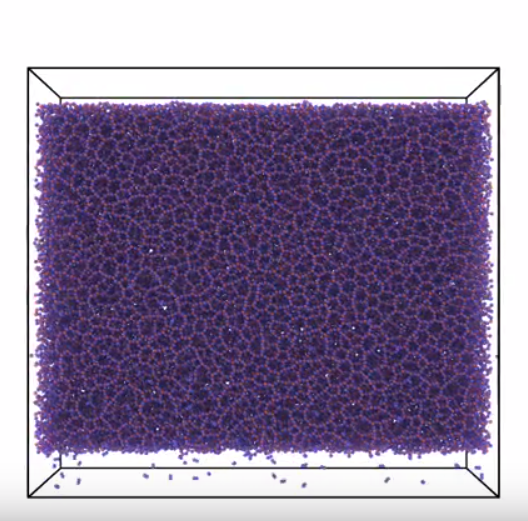
\includegraphics[width=0.3\textwidth,height=0.35\textwidth]{images/frac_prop1.PNG}\hspace{0.23\textwidth}%
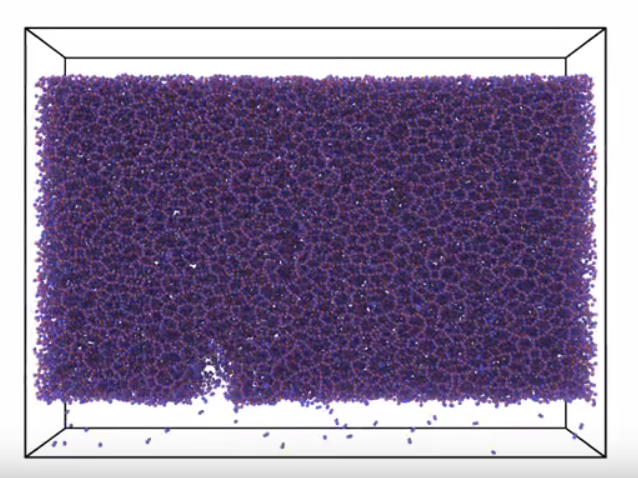
\includegraphics[width=0.375\textwidth,height=0.325\textwidth]{images/frac_prop2.PNG}\\[2em]
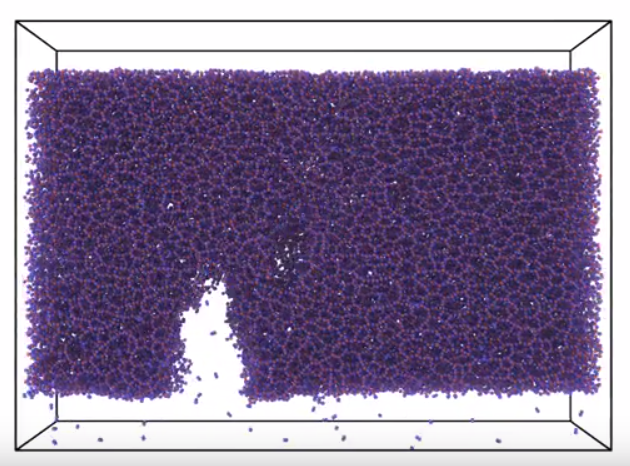
\includegraphics[width=0.4\textwidth,height=0.325\textwidth]{images/frac_prop3.PNG}\hspace{0.15\textwidth}%
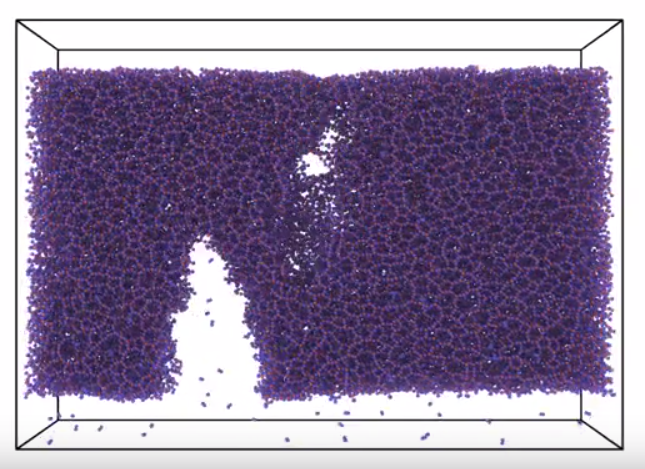
\includegraphics[width=0.45\textwidth,height=0.324\textwidth]{images/frac_prop4.PNG}\par
    \caption{Four snapshots showing the progression of an MD simulation of fracture propagation, in a 3D silicate glass sample. The material is loaded in uniaxial tension in the horizontal direction, with free surfaces in the two other directions.}
    \label{fig:crack_prop}
\end{figure}

Once the silicate glass is generated in this way, its dynamics may be simulated under a range of environmental conditions.  Figure~\ref{fig:crack_prop} shows several snapshots from an MD simulation representing a three-dimensional system of size approximately 15 $\times$ 15 $\times$ 4~nm$^3$, containing approximately 70,000 atoms, under uniaxial tension in the horizontal direction.  As the material is deformed, a fracture nucleates starting from the lower boundary.  The void then propagates upwards, while another void nucleates in the bulk.  Although these two voids do not coalesce during the 1~nanosecond time interval represented by the simulation, they would likely do so subsequently, leading to failure in the material.

An environmental condition of particular interest in simulating glass fracture dynamics is the presence of water, and its effects on fracture growth. Water weakens the bonds between silicon and oxygen, lowering the energy barrier for bond breakage. MD simulations have shown that silicates in contact with an aqueous environment are more susceptible to fracture, both at the boundary and within the bulk~\cite{chem_effects}. This suggests that chemical effects can complicate the mechanical stress effects in modeling fracture dynamics. Simulations of the chemical-mechanical effects on crack tips have shown differing rates of fracture propagation, as well as changes in fracture direction and stress distribution in the atoms in the process zone where fractures propagate. Other effects of water are corrosive and can take up to microseconds to be measurable~\cite{markpres}, far beyond the time scale of simulations such as the one shown in Figure~\ref{fig:crack_prop}.

\subsection{Machine Learning Methods} 

MD simulations require vast amounts of computation. For example, running the simulation shown in Figure~\ref{fig:crack_prop} takes approximately 10,000 CPU hours. Moreover, each MD simulation represents only one particular configuration of atoms, given a set of material properties such as Young's modulus and density. In order to obtain statistically reliable estimates of macroscopic material behavior, it would be necessary to simulate thousands if not millions of configurations consistent with these properties.  Clearly, this would render MD computationally prohibitive.

An attractive alternative is to use machine learning (ML) as a surrogate model.  In this approach, a supervised learning algorithm is trained using data from a moderately-sized set of MD simulation results.  Once trained, the algorithm can rapidly predict certain outcomes of the simulation simply from the initial state of the system.  Surrogate models have been used extensively in applications ranging from aircraft design~\cite{mack2007surrogate} to hydrology~\cite{razavi2012review}.  These models can be as simple as polynomial functions to which data points are fitted by regression, or can be complex statistical models with thousands of tunable parameters.  What they have in common is that they do not attempt to model an underlying physical mechanism but rather to reproduce, in an approximate sense, the results of the simulations that they imitate.

Recent years have seen a number of successful research efforts using ML, often coupled with graph theoretic approaches, to predict fracture properties in materials. Wang et al.~\cite{MLACrack} have studied the use of ML methods for predicting fatigue crack growth rates. Work originating in a 2016-17 CGU Math Clinic project~\cite{valera2018machine,TopSystem} has used supervised learning methods to provide rapid predictions of high-flow regions of a fracture network representing subsurface rock, based on graph centrality features and limited training data from high-fidelity simulations.  Ebrahem et al.~\cite{ebrahem2018influence} and Bauchy~\cite{bauchy} have demonstrated the role of topological features in glass networks, in order to understand how local atomic structure affects deformation and resistance to fracturing.  The use of ML in the design of new glasses has been the subject of further study~\cite{liu2019machine}.  Finally, in a 2017-18 CGU Math Clinic project, Schwarzer et al.~\cite{schwarzer2019learning,mudunuru2019} used a graph theoretic description of brittle materials, training a deep neural network to recognize the dynamics of fracture propagation based on data from discrete finite-element simulations.  These results suggest that ML methods can productively complement MD simulations, providing accurate surrogate models that can be trained to mimic the behavior of MD while using dramatically less computation time.


\section{Goals}
\label{sec: Goals}
The objective of our project is to develop supervised learning methods, trained on MD simulation data, that generate rapid predictions of where and when atomic-scale fractures occur in samples of silicate glasses under stress.  We aim to generate these predictions under multiple environmental conditions, and to validate them on existing MD simulation results.  Ultimately, we hope to relate our predictions to specific features characterizing local atomic structure, thus providing new insight into how this local structure leads to fracture and failure.

We separate our overall objective into the following two goals:

\begin{itemize}
\item \textbf{Goal 1:} \emph{Predict fracture nucleation events.} 

A nucleation event is where a new fracture, or void, emerges in the simulated system.  We aim to predict whether, based on the initial state of the system, a given atom lies on the boundary of a fracture at a certain later time in the simulation.  In order to do this, we assume that a nucleation event is primarily influenced by local atomic structure.  The definition of local could involve up to the $k$th neighbor of an atom, for some value of $k$.  The goal is to use network feature information of this kind to train a classifier to predict whether or not an atom ultimately forms part of a nucleation event.  We will also consider the closely related regression problem of estimating the probability that the atom forms part of a nucleation event.

\item \textbf{Goal 2:} \emph{Predict fracture propagation.} 

Fracture propagation is a continuing process of incorporating atoms into the fracture region, also known as the process zone.
Once a fracture nucleates at the surface or within the bulk of the material, it grows with the continued application of mechanical stress.  We aim to identify which new atoms will lie on the fracture's boundary, meaning the surface of a crack face, as it propagates.  Our goal is to train a supervised learning algorithm to learn the dynamics of fracture propagation from the full time series of feature values, so that it can then predict a time series from an initial state alone.
\end{itemize}






\chapter{Methods}
\label{sec: Methods}
Fracture at the atomic scale is a complex process controlled by the local structure of atoms, applied stress, forces between atoms and the strength of atomic bonds.  In order to predict the dynamics of the fracturing process, we will develop graph-based ML algorithms that learn from LAMMPS simulation data.


\section{Graph Representation}
SiO$_2$ may be represented as a network of silicon and oxygen atoms, connected with chemical bonds.  Predicting atomic scale fracture dynamics can therefore be understood as predicting the evolution of the graph that describes this network.

\subsubsection{Basic Graph Representation}

One straightforward graph representation of the atomic system is as follows.  Consider a graph $G =(V,E)$.  Let each element of the node or vertex set $V$ represent an atom, whether silicon or oxygen.  Let each element of the edge set $E$ represent a chemical bond between two atoms.  The resulting structure is illustrated in Fig.~\ref{fig:basic_graph}.  Note that in this representation, there is additional label information attached to each node, consisting of the atom type: Si or O.

\begin{figure}
\centering
\noindent
    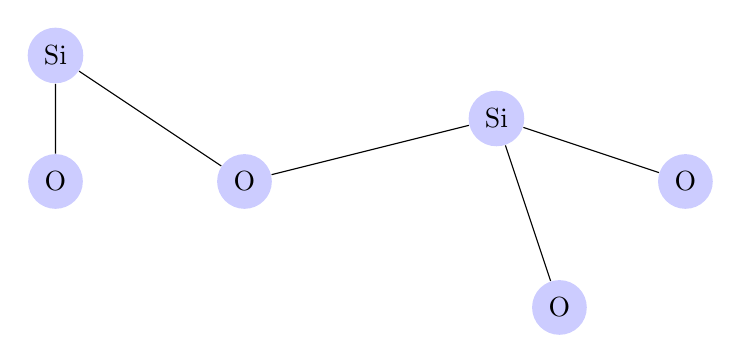
\begin{tikzpicture}
      [scale=.8,auto=left,every node/.style={circle,fill=blue!20}]
      \node (n6) at (1,10) {Si};
      \node (n4) at (4,8)  {O};
      \node (n5) at (8,9)  {Si};
      \node (n1) at (11,8) {O};
      \node (n2) at (9,6)  {O};
      \node (n7) at (1,8)  {O};
    
      \foreach \from/\to in {n6/n4,n4/n5,n5/n1,n2/n5,n6/n7}
        \draw (\from) -- (\to);
    
    \end{tikzpicture}
\caption{Basic graph representation, where nodes denote either silicon or oxygen atoms and edges denote bonds between atoms.}
\label{fig:basic_graph}
\end{figure}

As uniaxial stress is applied to the material, bonds can break and form, whereas atoms are conserved.  Thus, the vertex set remains constant, with size $|V|=n$ given by the total number of atoms in the system, whereas the edge set evolves in time.  We then define $E(t)$ to be the edge set at time step (snapshot) $t$, and $G(t) = (V,E(t))$ to be the graph at time step $t$.

There are significant benefits to having vertices whose identities do not change over the course of the simulation.  When predicting whether or not an atom ends up on the surface of a crack face, it is convenient to able to describe that atom by the same graph element at $t=0$ as at the time of prediction.  A drawback of this representation, however, is the resulting graph size for the samples that we will study.  Training an ML algorithm on graph inputs with 70,000 vertices may place excessive demands on computational resources.
    
\subsubsection{Reduced Graph Representation} 

An alternative graph representation is to consider only silicon atoms as nodes, and bonds through bridging oxygen atoms as edges.  Given the atomic content of SiO$_2$, this representation reduces the number of vertices approximately threefold, to 25,000 or less.  It also simplifies the encoding of Q$_n$ information, as a node with degree $n$ necessarily bonds to $n$ bridging oxygens, and thus forms a Q$_n$ unit.

Like the basic graph representation described previously, this reduced representation keeps the number of vertices constant.  On the other hand, it does not explicitly track bonds that are formed and broken at each time step. If a bond is broken in an Si--O--Si bridge, this representation will not distinguish between the case where the first bond, or the second bond, or both, are broken, although this may not be an issue if we are primarily interested in Si atoms on the crack face.  Similarly, the coordination number of an Si atom will not be given explicitly by node degree.  However, this information can, if needed, be encoded as feature information (see below).

\subsubsection{Topological Graph Representation}


We will also explore additional means of representing the network.  One possibility may be in terms of ring structure.  Ebrahem et al.~\cite{ebrahem2018influence} have studied medium-range order in silica glasses, expressed by the sizes of rings of alternating Si and O atoms, which correspond to cycles in the two graph representations discussed above. It has been observed that these ring size statistics can influence the tensile strength of SiO$_2$, with a flatter distribution of sizes accelerating the fracturing process, and a more sharply peaked distribution (larger number of medium-sized rings) delaying it. The intuition behind this observation is that large rings create large void in the material. And as tensile is applied, the void will be more likely to deform and eventually lead to fracture.

As a result, it is possible that, by letting vertices represent rings with vertex labels describing ring size, we may obtain useful predictions of fracture locations. This approach would provide a very significant reduction of graph size.  It would have the limitation, however, that the vertex set would not remain constant from one time step to the next.  As bonds break and form, the composition of the rings change, and it may be challenging to interpret what a particular $t=0$ ring becomes at a later time.


\section{Feature Description}
\label{subsec: Features}
Given a graph representation, we may associate features with the nodes (as well as, in principle, the edges) of the graph.  Our ML algorithm can use these features to describe data points in the training set, learning a function that maps feature values to an output label.  The challenge is to identify features that are likely to have predictive value for the output label of interest, namely whether a node is on the surface of a crack face.


The work of previous CGU Math Clinic projects~\cite{valera2018machine,schwarzer2019learning} on graph-based ML for fracture prediction has suggested that different categories of features can be useful. Some of these are quantities that describe physical properties of an atom.  Others are local topological measures, that describe the network structure in the immediate proximity of a node. Finally, there are global topological measures, that describe ``centrality'' properties quantifying the importance of a node to network processes on the network such as communication or flow.

We propose a range of candidate features that are meaningful both for the basic and for the reduced graph representations.  For other formulations, such as in terms of ring structure, further study will be needed to determine appropriate quantities.  Furthermore, not all features that we initially propose will be significant for model predictions.  After running our ML algorithms based on these features, we will perform feature analysis to determine which characteristics of the system play an important role in the accuracy of predictions.

\subsubsection{Physical Features}
\label{subsubsec: Physical Features}

\begin{itemize}
    
    \item \textbf{Cell volume:} A local density measure is given by the Voronoi diagram that partitions the system into polygonal cells surrounding each atom.  We define $v_i(t)$ to be the Voronoi cell volume of atom $i$ at time $t$.  These cell volumes can help our model understand which atoms are closely associated with fracture nucleation, by learning how and where volume increases.  When a fracture emerges, atoms neighboring it will have rapidly increasing cell volumes representing newly available space in the void.
    
    Note that while atoms on the boundary of a free surface can also have very large cell volumes, these volumes will already be large at $t=0$ and will typically not change as dramatically during the simulation.  A model that correctly learns the dynamics of cell volumes should therefore avoid mistaking the free surface for a fracture.

    \item \textbf{Atom displacement:} As fractures nucleate, atoms on its boundary may undergo more rapid displacement than do others.  Let $\mathbf{r}_i(t)$ be the vector representing the $(x,y,z)$ position of atom $i$ at time $t$. The physical displacement of an atom from one time step to the next is $\Delta \mathbf{r}(t)=\mathbf{r}_i(t)-\mathbf{r}_i(t-1)$.
    
    Of course, this feature is not defined at $t=0$.  However, for an ML algorithm that learns dynamics from a full time series, incorporating displacement as an explicit feature may be productive in training the algorithm on where and when fractures grow.

    \item\textbf{Stress tensor:} The virial stress tensor $\boldsymbol{\sigma}$ describes the local stress at each atom.  It may be the case that, prior to fracture growth, atoms that will ultimately form the fracture boundary undergo changes in values of their stress tensor components~\cite{elastic_fracture}. Note that, even in the absence of fracturing, considerable local fluctuations may occur in these values from one atom to the next.  Some form of spatial averaging may help in reducing these fluctuations.

    \item\textbf{Charge:} The emergence of fractures arises most directly from bond breaking.  The charge of an atom plays a crucial role in this.  As with the stress tensor components, we expect that atoms on a fracture boundary may, prior to fracture growth, exhibit characteristic changes in charge value.
    
    \item \textbf{Active atoms:} Over the course of the simulation, bonds break and new bonds form.  When a bond breaks, we define atoms that it previously connected to be active.  Likewise, when a new bond forms, we defines the atoms that it connects to be active.  Once an atom becomes active, it is considered active for the entire remainder of the simulation.
    
    It is natural to expect that being active is a necessary (but not sufficient) condition for an atom to be on the surface of a crack face.  As with atom displacement, this feature does not provide useful information at $t=0$, but could be productive in enabling an algorithm to focus on a subset of atoms of interest if it trains on a full time series.

\end{itemize}

\subsubsection{Local Topological Features}

\begin{itemize}
    \item \textbf{Coordination number:} The coordination number of an atom is the number of neighboring atoms to which it is bonded. Undercoordination and overcoordination could play a role in determining whether an atom will be on the boundary of a fracture.
    
    In our basic graph representation, the coordination number is equivalent to the degree of a vertex.  Even though it is implicit in the graph structure, however, there can be value in including it as an explicit feature for an ML algorithm to learn.
    
    In our reduced graph representation, the coordination number cannot be inferred from the graph at all, and must be included explicitly.

    \item\textbf{Number of bridging oxygens:} In a Q$_n$ unit, an Si atom is surrounded by $n$ bridging O atoms, each forming an Si--O--Si group.  The value of $n$ therefore supplies crucial network connectivity information. 
    
    In our reduced graph representation, the number of bridging oxygens is equivalent to the degree of a vertex.  Even though it is implicit in the graph structure (as with coordination number in the basic graph representation), ML algorithms may benefit from having it as an explicit feature.
    
    In our basic graph representation, this quantity would only be of direct use for those vertices that denote silicon atoms.  However, by setting it to a value of 0 for oxygen atoms, it could provide a means of distinguishing which type of atom a vertex represents: Si or O.

    \item\textbf{$k$th neighbor quantities:} A crucial assumption in our modeling approach is that structure beyond nearest-neighbor information can help in predicting fracture nucleation.  We therefore propose considering not only the number of bridging O atoms directly bonded to an Si atom, but also the number within a given number of bonds from an Si atom.
    
    In the reduced graph representation, a qualitatively similar quantity would be the following.  For an atom $i$ at time $t$, let $b^{(k)}_i(t)$ be the number of vertices whose path length to $i$ consists of at most $k$ edges. This defines a class of features for different values of $k$.  For $k=1$, $b^{(1)}_i(t)$ would simply be the vertex degree, i.e.,\ the number of bridging oxygens around $i$.  For increasing $k$, these features would consider local neighborhoods (around $i$) of increasing size.
    
\end{itemize}

\subsubsection{Global Topological Features}

\begin{itemize}
    
    
    \item \textbf{Eigenvector centrality:} The influence of a specific node on a network is described not only by local properties of the node.  For instance, a node may have high degree but still not play a central role in processes on the network such as flow or communication.  Eigenvector centrality is one way of quantifying a node's global influence.
    
    Given an adjacency matrix $\mathbf{A}$ for a graph, where element $A_{ij}=1$ if an edge connects nodes $i$ and $j$ and $A_{ij}=0$ otherwise, the eigenvector centrality $e_i$ of node $i$ is the $i$th component of the leading eigenvector of $A$.  It satisfies
    \begin{equation}
    \lambda_{\max}(\mathbf{A}) e_i = \sum_{j=1}^n A_{ij}e_j,
    \end{equation}
    where $\lambda_{\max}(\mathbf{A})$ is the largest eigenvalue of $\mathbf{A}$.  The recursive nature of this equation reflects the intuition that an influential node is one that links to other influential nodes.  Previous research on fracture networks has found that eigenvector centrality can help describe a node's influence on certain kinds of fracture behavior~\cite{santiago2016,valera2018machine}, suggesting that it could be a relevant feature for predicting fracture growth.
    
    \item\textbf{Betweenness centrality:} A further global measure of node influence is the number of paths in the network that pass through that node.  This reflects the node's importance in communication across the network, which is relevant when the effects of uniaxial stress are distributed over the network.  Betweenness centrality counts the fraction of geodesic paths (paths with fewest possible edges) that include a given node.
    
    If $\pi_{uv}$ is the total number of geodesic paths connecting node $u$ to node $v$, and $\pi_{uv}(i)$ is the number of such paths that pass through node $i$, then the betweenness centrality of node $i$ is given by
    \begin{equation}
    \beta_i = \sum_{\substack{u,v = 1 \\ u\neq i\neq v }}^n \frac{\pi_{uv}(i)}{\pi_{uv}}.
    \end{equation}
    If the simulated sample had free boundary conditions in the direction of loading ($x$ direction), it is possible that relevant paths would only be those between a node $u$ along the left-hand boundary and a node $v$ along the right-hand boundary.  Since we are instead working with periodic boundary conditions in the $x$ directions, we will explore other possible ways of limiting the paths counted in the sum above.
\end{itemize}

\section{Quantities of Interest}

In this project, we will use a supervised learning technique. To train a supervised machine learning model, examples of input-output pairs are needed. Each of these pairs have the input and the corresponding desired output, which we call the ground truth. In this section, we discuss three potential definitions of ground truth, which are dummy indicator of fracture face, cell volume as indicator of fracture face, and dummy indicator of large-sized ring.

\subsection{Dummy Indicator of Fracture Face}

The most straightforward way of defining ground truth is a dummy indicator variable $\phi_i(t) \in\{0,1\}$, specifying whether or not an atom $i$ is part of a fracture at time $t$. Given a system with $n$ atoms, $\boldsymbol{\phi}(t)$ is a binary vector of length $n$. An important consideration, however, is that the simulation data described in previous sections does not directly give ground truth information. Instead, the ground truth must be extracted from the simulation output.

A fracture involves the creation of a void in the material. When stress is applied uniaxially, bonds break and form.  As a fracture nucleates, some atoms are on the boundary of the emerging void, while others are compressed into denser regions. Consequently, we define the ground truth using a local density measure closely related to the first of the physical features described above.  Consider the Voronoi cell volume $v_i(t)$ of atom $i$ at time $t$.  When this volume exceeds a certain threshold, we consider atom $i$ to be part of a fracture event.  Figure~\ref{fig:crack_vol} highlights in red the atoms that would be identified in this way with a fixed threshold value, on a snapshot from a dry simulation with fully periodic boundary conditions.

    \begin{figure}
    \centering
    \noindent
    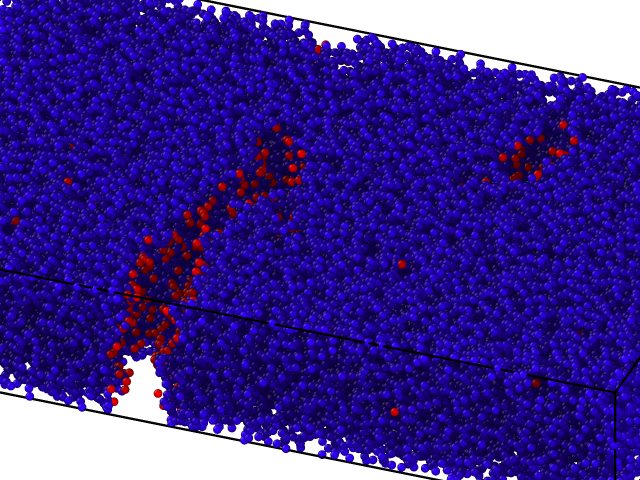
\includegraphics[width=8cm, height=6cm]{crack_vol.png}
    \caption{Atoms in red are those with Voronoi cell volume $v_i>0.042$~nm$^3$.  The voids represent fractures.}
    \label{fig:crack_vol}
    \end{figure}
    
In order to establish the ground truth, we will set the threshold value for a given time $t$ to be equal to three standard deviations above the mean Voronoi cell volume at that time.  Thus, we define a standardized cell volume and test whether it is greater than 3:
    \begin{equation}
    \hat{v}_i(t) = \frac{v_i(t) - \mu_v(t)}{\sigma_v(t)} > 3,
    \end{equation}
where $\mu_v(t)$ is the mean and $\sigma_v(t)$ is the standard deviation of $v_i(t)$ over all $i\in\{1,\dots,n\}$.  Note that in the postprocessed nucleation data supplied with the simulations, this is equivalent to testing whether the quantity in the field {\tt nuc\_v} exceeds 1.

Because of the effects of free surfaces discussed in Section~\ref{subsubsec: Physical Features} above, $v_i(t)$ must be modified to disregard cell volumes that are large because they are on the boundary of a surface rather than a fracture.  Since these cell volumes do not significantly change over time, we define a new quantity that subtracts out the $t=0$ value, $v'_i(t) = v_i(t)-v_i(0)$, and instead test whether
\begin{equation}
    \label{eqn: cell volume}
    \hat{v}'_i(t) = \frac{v'_i(t) - \mu_{v'}(t)}{\sigma_{v'}(t)} > 3.
\end{equation}
The ground truth can then be defined:
\begin{equation}
    \label{eqn: ground truth}
    \phi_i(t) = \begin{cases}
      0 & \text{if }\hat{v}'_i(t) \le 3 \\
      1 & \text{if }\hat{v}'_i(t) > 3 \\
    \end{cases} 
\end{equation}

We will apply two further corrections to $\phi_i(t)$, to limit the case of false negatives (where atoms on the boundary are identified as $\phi_i(t)=0$) as well as false positives (where atoms not on the boundary of a fracture are identified as $\phi_i(t)=1$).

The false negative case occurs when an atom is at the boundary of a fracture, but is surrounded by a sufficient number of other nearby atoms that its Voronoi cell volume does not extend out into the void.  To account for this, we will consider a small neighborhood around each positively identified atom $i$.  Any other atom whose path length to $i$ consists of fewer than a small number of edges (such as 2 or 3) will be considered to be on the boundary as well.

The false positive case occurs early in the simulation, prior to nucleation, when the standard deviation $\sigma_{v'}(t)$ is very small, and atoms can be identified as positive purely due to spatial fluctuations in density.  To reduce this problem, we use the fact that an atom on the boundary of a fracture at time $t$ is expected to remain on the boundary of a fracture for the remainder of the simulation.  If an atom is positively identified, we will test whether it remains positively identified for the majority of the remaining simulation times.  If not, it will not be considered to be on the boundary.

\subsection{Cell Volume as Indicator of Fracture Face}

We propose an alternative way to extracting information from simulations on whether an atom is at a fracture boundary, and then training our algorithms using this ground truth.  Instead, we can simply adopt the cell volumes as ground truth, and train our algorithms to predict this.  Our predictions may then be post processed using Equations~(\ref{eqn: cell volume}) and (\ref{eqn: ground truth}) to determine which atoms are at fracture boundaries.  This could have the advantage of providing a more objective prediction, but involves solving a regression problem rather than merely a classification problem.

\subsection{Indicator of Large Sized Ring}

Under the assumption that large-sized ring, especially ring of size 20, is a potential solid indicator of fracture nucleation, we can also define the ground truth as a dummy indicator variable $\phi_i(t) \in\{0,1\}$, specifying whether or not an atom $i$ has ever been part of a large-sized ring during all simulation steps. The advantage of this definition is that in such a way, this indicator is less arbitrary. However, the disadvantage is that the number of large rings is very small compared to other smaller-sized rings. For example, in one simulation, only 423 out of around 70000 atoms are part of a 20-sized ring. This worsens the imbalanced classes issue and thus creates a modelling challenge to tackle this problem.


\section{Machine Learning Methods}

The objective of this project is to produce a surrogate model of the molecular dynamic simulations using supervised machine learning techniques. We propose to address our two goals listed in Section~\ref{sec: Goals} with two methods, respectively. First, we will use ensemble methods such as random forest to predict nucleation at a fixed future time step, given feature information at $t=0$.

Second, we will use a recurrent neural network (RNN) with the long-short term memory (LSTM) mechanism, to learn the dynamic process of fracture propagation.

\subsubsection{Random Forest for Predicting Fracture Nucleation}

%Random forest. Boosting, bagging. 
For the purpose of determining whether or not a node is associated with a fracture, we will implement ensemble-based ML methods. The goal of ensemble methods is to take predictions made by a subset of features, and combine them into one single learned estimator. With our feature set being quite large, ensemble methods may be a useful means to predict fracture labels. 

Core ensemble methods include bagging (bootstrap aggregating) and boosting. A ``bagged'' random forest method is generated by creating a tree from features randomly drawn with replacement. 
% Since our representation is graph-like these trees make sense logically. 

Our bagging algorithm will work as follows:

\begin{enumerate}
\item Take training set $T$ with $N$ features.
\item Create $n$ models $\{L_1,\dots,L_n\}$.
\item For model $L_i$, create a training set by choosing $d_i<N$ features from $T$ with replacement, and train the model.
\item Determine the output of the algorithm by majority vote among the $n$ models.
\end{enumerate}

Adaboost (adaptive boosting), on the other hand, is a boosting method that learns from previous mistakes made during training. By doing so, the model can increase the weights of incorrectly predicted points from the training data.

Our boosting algorithm will work as follows:

\begin{enumerate}
    \item Initialize weights for each individual feature.
    \item Train a classifier on each individual feature.
    \item Find the weighted misclassification (error) rate.
    \item Update feature weights based on this error.
    \item Repeat until error is minimized.
\end{enumerate}


\subsubsection{Fracture Propagation}
%RNN, 

\begin{figure}[!b]
    \centering
    \noindent
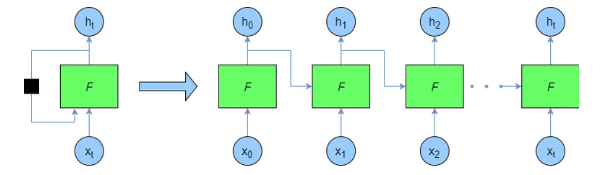
\includegraphics[width=12cm , height = 5cm]{rnn.PNG}
    \caption{Representation of a Recurrent Neural Network}
    \label{fig:rnn}
\end{figure}

Due to the dynamical nature of our graph changing over each time step, we will be implementing an RNN to predict the ground truth at each time step. An illustration of the basic RNN architecture is shown in Figure~\ref{fig:rnn}.  The main idea behind an RNN is that it trains on an entire time series, learning the dynamics of a process which it stores using a ``memory'' of internal states.  The LSTM mechanism is a refinement of this memory, allowing the neural network to give added weight to information learned in more recent time steps.

The training input to our RNN will be a time series of graphs based on simulation data, where nodes will be labeled with the full set of feature values described in Section~\ref{subsec: Features}.  For every time $t$, the RNN uses the (appropriately weighted) information from that and all previous times to output feature and ground truth values for time $t+1$.  These are compared with simulation results, from which a loss function is calculated and the internal neural network weights are updated.

Once the RNN is trained and its weights are set, it is used for prediction.  Unlike in the training phase, the input in the prediction phase is simply the $t=0$ feature values.  The output is a time series of graphs, giving the full predicted evolution of features and ground truth.

Recall that certain of our features, such as atom displacement and active atoms, are undefined at $t=0$ and thus meaningful only as part of the training process.  Others, however, are well-defined at any individual time step.

\subsubsection{Algorithmic Architecture}


The proposed architecture is as follows:

\bigskip

\begin{center}
\tikzstyle{decision} = [diamond, draw, fill=blue!20, 
    text width=4.5em, text badly centered, node distance=3cm, inner sep=0pt]
\tikzstyle{block} = [rectangle, draw, fill=blue!20, 
    text width=5em, text centered, rounded corners, minimum height=4em]
\tikzstyle{line} = [draw, -latex']
\tikzstyle{cloud} = [draw, ellipse,fill=red!20, node distance=3cm,
    minimum height=2em]
    
\begin{tikzpicture}[node distance = 2cm, auto]
    % Place nodes
    \node [block] (init) {MD Simulation Data};
    \node [block, below of=init] (features) {Extracted Features};
    \node [block, below of=features] (training) {Training Set};
    \node [block, left of=training, node distance=3cm] (test) {Test Set};
    \node [block, right of=training, node distance=3cm] (validate) {Validation Set};
    \node [decision, below of = training] (RF) {Random Forest};
    \node [decision, below  of = test] (rnn) {LSTM};
    \node [cloud, below of = RF] (out) {Surrogate Model};
    %\node [cloud, below of= RF, node distance=3cm] (pof) {RF Output};
    %\node [cloud, below of= rnn, node distance=3cm] (rnnout) {RNN Output};

    % Draw edges
    \path [line] (init) -- (features);
    \path [line] (features) -- (validate);
    \path [line] (features) -- (training);
    \path [line] (features) -- (test);
    \path [line] (training) -- (RF);
    \path [line] (training) -- (rnn);
    \path [line] (rnn) -- (out);
    \path [line] (RF) -- (out);
    \path [line] (validate) |- node [near end] {} (out);
\end{tikzpicture}
\end{center}

\begin{enumerate}
    \item Analyze and determine features from the MD data.
    \item Extract the features and prepare data for training.
    \item Split the dataset into three sets: training, validation, and test
    \item
    \begin{enumerate}
        \item Train the training set using Random Forest to predict which atoms are part of a fracture.
        \item Train the data using LSTM to predict fracture evolution.
    \end{enumerate}
    \item Validate surrogate model using validation set.
    \item Feature analysis. Fine tune features which are deemed most important. 
    \item Finalize surrogate model on test set. 
\end{enumerate}

\chapter{Preliminary Results}
\label{sec: Preliminary Results}
\section{Data Used}
\subsection{Initial Data}
%The initial architecture has been developed using a data package from LANL for a two-crack system. Data for 250 time steps was provided, with failure occurring at step 52. While useful for testing purposes, this mesh was much coarser than those of the true systems. Hence, for training the network, we used more representative systems of standard HOSS output.

Our preliminary investigation was localized to one LAMMPS simulation run. The data used contained information on bonds, atoms and rings, under the fully periodic condition.

\subsection{Training Data}
At the moment, data from one fully periodic simulation is used to train the base case model presented below.  Ultimately, we plan to generalize across different numbers of simulation to create a more sophisticated model and improve predicting accuracy. 

The features we use include cell volume, number of bonds and maximum ring size at initial time step. The label is the dummy indicator of whether or not a certain atom has ever been part of a 20-sized ring during the whole time steps.

\section{Graph Representation}

\subsection{Creation}The first milestone was to implement the basic graph representation in Python. Using the NetworkX library we were able to reconstruct the simulation in Python where a node is an individual atom, Si or O, and an edge is a bond between atoms. With this graph we were able to not only visualize our simulation at a more local window but we are able to create different measures, such as centrality. 

\subsection{Correlation Between Features}
After the graph had been created are now able to take a look at how the features of the atoms play a role within the structure and how they correlate with other quantities of interest within the system. One such structure is the role bridging oxygen play within the global structure of the simulation. 


\section{Results}
In this section, we presents the preliminary results we obtained from base case toy models, which are Logistic Regression and Support Vector Machine with imbalanced class.

\subsection{Logistic Regression}
Logistic Regression is a static model that we use to predict the labels with probabilities of the underlying classes. However, due to imbalanced class, the model ignores the false negatives and predicts all the labels to be negative to obtain a high accuracy. 

\subsection{SVM with imbalanced class}
To tackle the problem of imbalanced class, we also implemented a Support Vector Machine model with a penalty,$c=1$, on the imbalanced classes. The model obtains an accuracy of 66\% and an area under the AUROC curve of 0.58.


\section{Remaining Milestones}
Now that this complex problem has been defined and initial investigations are complete, the remaining milestones for the Spring semester are to begin and complete the machine learning framework for predicting the project goals. 

\begin{enumerate}
\item Additional features extracted from the MD simulation data to add to training set.
\item Ensemble classification method as well as recurrent neural network.
\item Refine and add complexity to the network.
\end{enumerate}


\section{Deliverable Status}
\begin{enumerate}
\item Graph representation implemented in Python.
	\begin{itemize}
		\item Basic graph representation completed. More complex representations currently being investigated. 
	\end{itemize} 
\item Feature extraction from the MD simulation data to create training set.
	\begin{itemize}
		\item Raw features from MD simulation data extracted and analzyed. Advanced measures and feature correlation in progress. 
	\end{itemize} 
\item Midterm presentation.
	\begin{itemize}
		\item Complete, November 20, 2019.
	\end{itemize} 
\item Mid-year report.
	\begin{itemize}
		\item Complete, December 16, 2019.
	\end{itemize} 
\item  Journal  article  on  graph-theoretic  machine  learning  approach  forpredicting fracture dynamics, submitted to peer-reviewed journal.
	\begin{itemize}
		\item Forthcoming, Spring 2019.
	\end{itemize} 
\item Final presentation.
	\begin{itemize}
		\item Forthcoming, Spring 2019.
	\end{itemize} 
\item Final report.
	\begin{itemize}
		\item Forthcoming, Spring 2019.
	\end{itemize} 
\end{enumerate}

\iffalse
\subsection{Crack Identification}
In converting HOSS FDEM output to graph form, recall that we follow two rules to preserve the integrity of the fracture network:
\begin{itemize}
	\item Edge crack identification must remain fixed over time.
 	\item Crack identity must be preserved through coalescence.
\end{itemize} 
By preserving the identification of each crack through both time and coalescence, we provide the necessary index for identification and tracking of each crack across all time steps, as well as correct attribution of feature metrics to the appropriate locations.
          
\subsection{Graph Data Matrices}
In order to set up the Graph Convolutional Neural Network architecture, we need to define the metrics used in the Adjacency and Feature matrices.\\
Distance Metrics:
        \begin{itemize}
        \item Coalescence (binary)
        \item Tip Intersect Distance  
        \item Shortest Euclidean Distance
        \item Minimum Damage Path
        \end{itemize}       
Features:
    \begin{itemize}
	\item Maximal horizontal projected crack tip Euclidean length
	\item Maximal vertical projected crack tip Euclidean length 
	\item Crack extreme tip Euclidean length
    \item Maximal Crack path Euclidean length between two tips
    \item Total path length including all crack tips
    \item Total crack damage
    \item Max tip stress
    \item Mean tip stress
	\end{itemize}
    
Functions were created to calculate and extract this data from HOSS simulation data to create graph data matrices for each HOSS time step.  

\section{R-GCN Setup}
The second milestone is to construct a working algorithm and model from the graph representation to predict the behavior of the fracture network over time. We accomplish this by using the Keras library for Python as a basis for building our RNN \cite{chollet2015keras}. The model simultaneously outputs predictions for both the features and each distance metric while following precisely the architecture presented in section 3.4. The implementation of the graph convolutional layer is taken from \cite{kipf2016semi}.

\section{Results}

As mentioned, our preliminary results come from training on three twenty-crack systems. In order to augment training data and increase the generalization ability of the network, we randomly take slices of 25 time steps. This allows for the network to learn from varying starting points and works to prevent overfitting. Also, the features are normalized across feature type before training using a normalizing matrix. Given that some features, such as total crack damage, can become large near the end of the system this serves to condense values to a far smaller range and enable better learning. Ultimately, the feature predictions can be transformed back to their original scale through the same normalizing matrix from the training data.

Our goal is for our network to be able to generalize, to predict systems on which it has not been trained. However, for these initial tests, we perform the more simple task of predicting the evolution of one of the three crack systems from time step 0 to the final time step. As described in the methods section, there will first be a prediction for time step 1 given input at time step 0, then for time step 2 given input at time steps 0 and predicted output from time step 1 and so on. This will test the general ability of the architecture to learn and find patterns.

\begin{figure}[!htb]
\centering
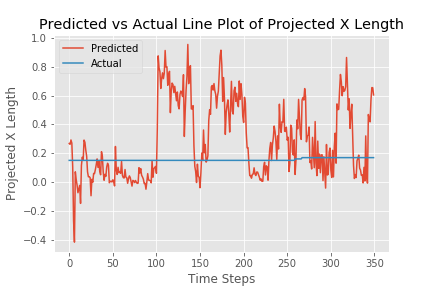
\includegraphics[width=0.8\textwidth]{images/Projected_X_Length_compare_transformed}
\caption{Plot comparing the predicted values against true values for projected $x$ length of crack 19.}
\label{fig:proj_y}
\end{figure}

\begin{figure}[!htb]
\centering
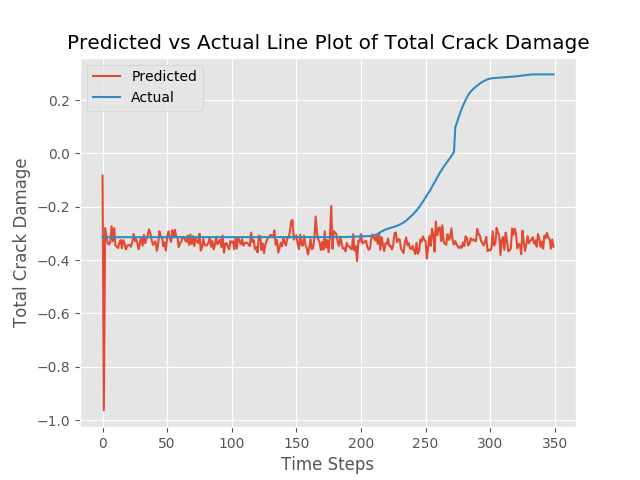
\includegraphics[width=0.8\textwidth]{images/Total_Crack_Damage_compare}
\caption{Plot comparing the normalized predicted values against the normalized true values for total crack damage in crack 4.}
\label{fig:tot_dam}
\end{figure}

In figures \ref{fig:proj_y} and \ref{fig:tot_dam}, selected results for feature prediction are presented. In figure \ref{fig:proj_y},we plot the projected $x$ length vs.\ time, for a simulated system with total size of 3 in the $x$ direction and 2 and in the $y$ direction.
%The spatial scale of the material in this simulation run is 3 by 2( Total X length 3, Y length 2).
The actual projected $x$ length does not change until time step 200.  Many of the features in a given simulation are essentially constant, and thus in our limited training, the model has overfit to these examples. This is illustrated in figure \ref{fig:tot_dam}, where the damage changes near the end of the simulation, yet our network is unable to predict the change.

As the output from HOSS is not deterministic, the comparison between distributions of crack features is more meaningful than feature comparisons on specific cracks. In figure \ref{fig:mean_proj_x_length}, we plot our prediction for the mean projected $x$ length of all cracks, along with the actual mean projected $x$ length. The band represents plus and minus one standard deviation of the crack features. As we can see, the mean and variance in our prediction is tracking the actual when the cracks start growing quickly around time step 220.

Ultimately, these preliminary results showed us that the network has the ability to learn. It does not predict each feature perfectly, yet it does give meaningful predictions for distributions over all cracks in the system. These results leave us optimistic for future results given additional network refinement and more substantial training.

\begin{figure}[!htb]
\centering
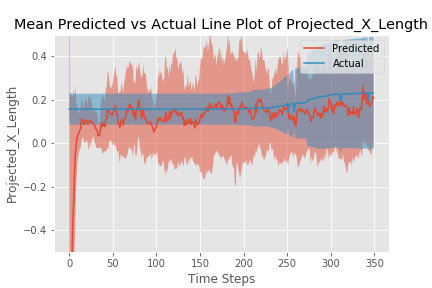
\includegraphics[width=0.8\textwidth]{images/Projected_X_Length_mean_variance_compare_ylim_test}
\caption{Plot comparing the mean predicted values against mean true values for projected $x$ length of all cracks. Shaded bands show one standard deviation above and below mean.}
\label{fig:mean_proj_x_length}
\end{figure}

\section{Remaining Milestones}
The two remaining milestones serve as goalposts for the second half of the CGU Math Clinic year:
\begin{itemize}
\item Determine the importance of different crack features for the prediction of the evolution of the fracture network.
\item Refine and add complexity to the network (i.e.,\ additional convolutional filters, layered graph convolution, compare effectiveness of spectral clustering graph convolutions versus standard graph convolutions).
\end{itemize}



\section{Deliverable Status}
\begin{enumerate}
\item Keras implementation of proposed architecture, coded in Python.
	\begin{itemize}
		\item In progress.
	\end{itemize} 
\item Full documentation of code in iPython Notebook.
	\begin{itemize}
		\item In progress. On track to be finalized along with final code.
	\end{itemize} 
\item Midterm presentation.
	\begin{itemize}
		\item Complete, November 14, 2017.
	\end{itemize} 
\item Mid-year report.
	\begin{itemize}
		\item Complete, December 18, 2017.
	\end{itemize} 
\item Journal article on the dynamic prediction of the fracture of brittle material using deep learning, submitted to peer-reviewed journal.
	\begin{itemize}
		\item Forthcoming, Spring 2018.
	\end{itemize} 
\item Final presentation.
	\begin{itemize}
		\item Forthcoming, Spring 2018.
	\end{itemize} 
\item Final report.
	\begin{itemize}
		\item Forthcoming, Spring 2018.
	\end{itemize} 
\end{enumerate}
\fi


%%% Appendices.

%%% The appendices are delineated with the \appendix command.
%%% Individual appendices are begun with the standard \chapter or
%%% \section commands.
%\appendix
%\chapter{Appendix}
%\input{Appendix}

%\backmatter

%%% Bibliography.

%%% Depending on your field, it may or may not be appropriate to list
%%% references for which you haven't included specific citations.  If
%%% your field sanctions such practices, or if you just want to get an
%%% idea of what you have in your bibliography file, you can include
%%% everything with the \nocite{*} command.          

%%% The appearance of your bibliography and citations in your text are
%%% defined by a combination of any bibliography-related LaTeX
%%% packages (such as natbib, harvard, or chicago) and the particular
%%% bibliography style file that you load with the \bibliographystyle
%%% command.  Bibliography-style files end in .bst; you can find them
%%% by searching your file system using whatever tools you have for
%%% doing searches.  (On most modern Unices, ``locate .bst'' will give
%%% you an idea of what's available.)

\bibliographystyle{IEEEtran}

\small

\bibliography{Bibliography}

\end{document}
